\documentclass[a4paper, 10pt, twoside]{article}
\usepackage[left=2cm, right=2cm, top=2cm, bottom=3cm]{geometry}
\usepackage{amsmath}
\usepackage[shortlabels]{enumitem}
\usepackage{bbold}
\usepackage{cases}
\usepackage{systeme}
\usepackage{graphicx}

\begin{document}

\title{Machine Learning - Theoretical exercise 4}
\author{T\'eo Bouvard}
\maketitle

\section*{Problem 1}
\begin{enumerate}[a)]
    \item We have the same number of training samples for classes $\omega_1$ and $\omega_2$, thus the prior probabilities are equal for both classes i.e. $P(\omega_1)=0.5$ and $P(\omega_2)=0.5$

          \begin{center}
              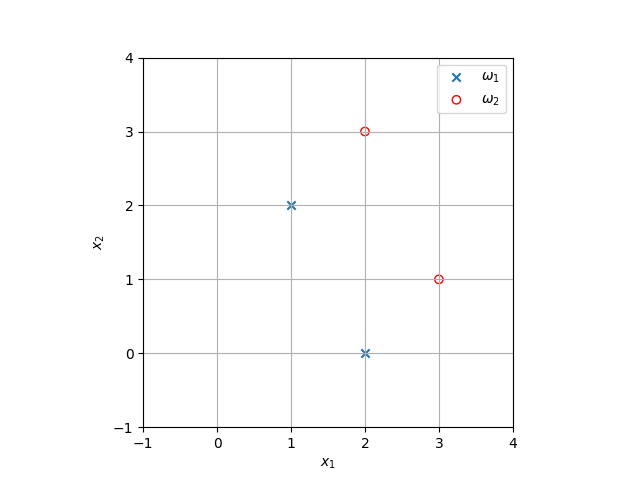
\includegraphics[width=0.5\textwidth]{graph1.png}
          \end{center}

    \item We compute $\theta$ according to the LS-method.
          \begin{align}
              \theta = (X^TX)^{-1}X^Ty
          \end{align}
          where
          \begin{align*}
              X =
              \begin{bmatrix}
                  1 & 2 & 1 \\
                  2 & 0 & 1 \\
                  3 & 1 & 1 \\
                  2 & 3 & 1 \\
              \end{bmatrix}^T
               &  &
              y =
              \begin{bmatrix}
                  1 \\ 1 \\ -1 \\ -1
              \end{bmatrix}
          \end{align*}
          The steps to solve this equation are shown below.
          \begin{align*}
              X^TX           & =
              \begin{bmatrix}
                  18 & 11 & 8 \\
                  11 & 14 & 6 \\
                  8  & 6  & 4 \\
              \end{bmatrix} \\
              (X^TX)^{-1}    & =
              \begin{bmatrix}
                  18 & 11 & 8 \\
                  11 & 14 & 6 \\
                  8  & 6  & 4 \\
              \end{bmatrix} \\
              (X^TX)^{-1}X^T & =
              \begin{bmatrix}
                  -\frac{1}{2} & -\frac{1}{6}   & \frac{1}{2}  & \frac{1}{6}   \\
                  0            & -\frac{1}{3}   & 0            & \frac{1}{3}   \\
                  \frac{5}{4}  & -\frac{13}{12} & -\frac{3}{4} & -\frac{7}{12} \\
              \end{bmatrix} \\
              \theta         & =
              \begin{bmatrix}
                  -\frac{4}{3} \\
                  -\frac{2}{3} \\
                  \frac{11}{3} \\
              \end{bmatrix} \\
          \end{align*}
          To determine the decision boundary, we find the root of the discriminant function.
          \begin{align*}
              g(x) = 0                                              \\
              -\frac{4}{3} x_1 - \frac{2}{3} x_2 + \frac{11}{3} = 0 \\
              x_2 = -2x_1 + \frac{11}{2}
          \end{align*}
          \begin{center}
              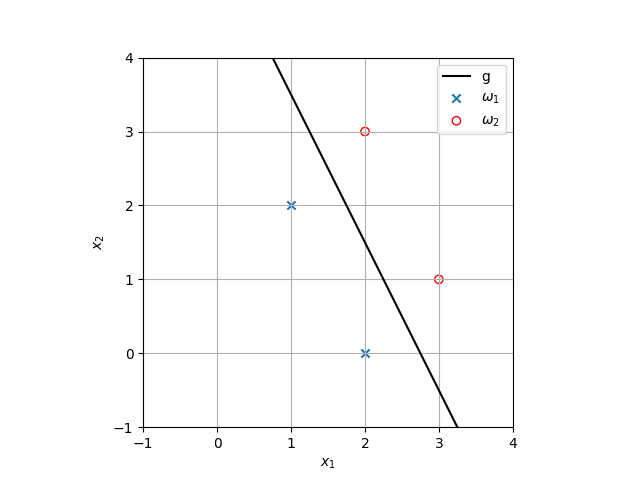
\includegraphics[width=0.5\textwidth]{graph2.png}
          \end{center}

    \item If we set $y_4=-0.5$, we reduce the weight of the fourth training sample, which modifies $\theta$.
          \begin{align*}
              \theta' =
              \begin{bmatrix}
                  -\frac{5}{4} \\
                  -\frac{1}{2} \\
                  \frac{27}{8} \\
              \end{bmatrix}
          \end{align*}
          Because $\theta' \neq \theta$, the decision boundary also changes.
          \begin{align*}
              g'(x) = 0                                             \\
              -\frac{5}{4} x_1 - \frac{1}{2} x_2 + \frac{27}{8} = 0 \\
              x_2 = -\frac{5}{2} x_1 + \frac{27}{4}
          \end{align*}
          \begin{center}
              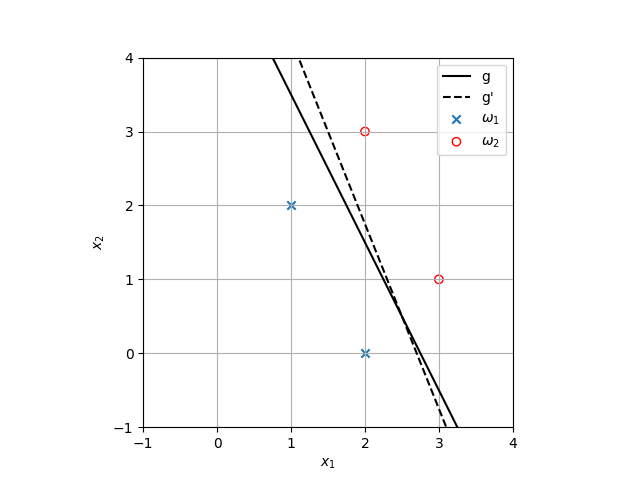
\includegraphics[width=0.5\textwidth]{graph3.png}
          \end{center}
          We can see that decreasing the weight of a training sample moves the decison boundary closer to it.

    \item We now compute $\theta$ with the LMS-method. For the sake of clarity, we will note the threshold value $\tau$, the learning rate $\mu$
\end{enumerate}


\end{document}
